\chapter{Il Dust Attack}
Tra i molteplici attacchi all'anonimato di Bitcoin, un attacco interessante é il Dust Attack, chiamato anche ``Forced reuse address" \cite{dst_att_def}. Il Dust Attack é una nota tecnica di de-anonimizzazione il cui obiettivo é capire che certi address appartengano al medesimo wallet.

In questa tesi:
\begin{itemize}
\item Definiremo il concetto di dust;
    \item Presenteremo le modalità più comuni con cui viene speso il dust, in particolare analizzeremo se e quanto possa essere efficace un Dust Attack mostrando gli effetti del dust sulla de-anonimizzazione degli address e dei relativi wallet;
    \item Descriveremo alcuni pattern interessanti che sono stati individuati e che potrebbero essere messi in relazione con il  Dust Attack.
\end{itemize}

Poiché il Dust Attack sfrutta l'utilizzo degli importi dust, é importante quindi spiegare cosa sia il dust e in generale quali possano essere i suoi possibili impieghi.

\section{Definizione del dust}
Il dust é una piccola quantità di criptovaluta presente in un UTXO sotto i limiti minimi di scambio, che chiariremo in seguito. Per definire il valore del dust é necessario fare alcune considerazioni.

Nelle transazioni di Bitcoin, generalmente, l'importo totale di input non viene speso completamente in output ma parte di esso viene inviato ai miners come fee. Formalmente la fee di una transazione, raccolta dai miners come ricompensa per includere la transazione in un blocco, é definita come:
\begin{center}
    $fee = \sum_{i=0}^{\#inputs} importo(input_i) - \sum_{j=0}^{\#outputs} importo(output_j)$
\end{center}
La fee quindi non é altro che la differenza tra l'importo totale di input e l'importo totale di output, e assume valori $\ge 0$. In generale la fee viene stabilita autonomamente dal creatore della transazione per incentivare i miners a validare la transazione stessa. Più la fee scelta é proporzionalmente alta, e più i miner guadagneranno nel validare la relativa transazione, rendendo la transazione prioritaria e quindi validata più in fretta.

Tuttavia, per convenzione, esiste una fee minima, denominata \textit{minimum relay fee}, che una transazione si suppone pagare affinché un qualsiasi nodo della rete peer-to-peer inoltri quella transazione agli altri nodi della rete. Questo valore non é prefissato ma varia piuttosto nel tempo in base allo stato della rete e all'andamento del suo valore. 

Nella comunità Bitcoin, spesso nuove convenzioni e comportamenti suggeriti sono pubblicati attraverso il client ufficiale, Bitcoin Core \cite{btccore}, poiché rimane ancora oggi il client più diffuso nella rete.  Tale client ha introdotto una convenzione, definita ``dust limit", che va rispettata per mantenere lo stato di transazione standard, cioé quelle transazioni che i nodi sono suggeriti accettare ed inoltrare ad altri nodi.

Lo scopo é quello di considerare non-standard le transazioni che includono degli output dust proprio perché costerebbe di più per il destinatario spendere l'importo dust rispetto al valore dell'output creato. Infatti un importo dust non può essere speso da solo in una transazione standard, poiché minore della \textit{minimum relay fee}, perciò deve essere necessariamente aggregato ad altri input.

In generale un valore dust consuma in fees un valore maggiore di quello scambiato. Questo di fatto lo rende razionalmente non spendibile, poiché il destinatario dovrebbe spendere più di quanto riceverebbe per ottenerlo. L'output però rimane tecnicamente spendibile e quindi deve essere mantenuto nell'UTXO, appesantendo inutilmente la struttura dati con valori inutili.

Il limite attuale é di 546 satoshi \cite{BtcDev}. Quindi tutti gli importi minori di 546 satoshi sono definiti \textbf{dust}.

\section{Possibili utilizzi del dust}

Gli usi del dust possono essere molteplici. Per esempio può essere utilizzato per effettuare degli stress test della rete Bitcoin, proprio perché permette di generare tante transazioni con molti output ad un basso costo complessivo. In questo caso il costo é determinato principalmente dalla fee della transazione e non tanto dagli output. Se consideriamo che il valore di 1 satoshi, unità minima di Bitcoin, vale meno di due centesimi di euro al momento (Novembre 2022), é possibile generare una transazione con 1000 output dust, 1 satoshi ciascuno, con meno di venti centesimi (fee esclusa).

In generale, dato l'irrilevante valore economico del dust, viene spesso usato per ottenere effetti laterali, diversi dal semplice scambio di valore. Nel seguito mostriamo tre esempi interessanti di tale uso del dust: la notifica dell'esito di scommesse nel servizio di gambling Satoshi Dice, la scrittura di dati arbitrari tramite lo script OP\_RETURN ed il Dust Attack.

\subsection{Satoshi Dice}
Satoshi Dice é un noto ``gioco di scommesse basato su blockchain" nato nell'Aprile 2012 \cite{SD}. A differenza dei tradizionali software di gioco online, le scommesse con Satoshi Dice possono essere inviate senza accedere ad un sito Web né eseguire alcun software client. Per giocare, viene effettuata una transazione Bitcoin a uno degli address resi pubblici da Satoshi Dice, caratterizzato da probabilità di vincita e quindi di pagamenti diversi.

Per essere meglio riconoscibili, tutti gli address resi pubblici da Satoshi Dice sono \emph{vanity address}. Un vanity address é un normale address Bitcoin con le stesse funzionalità di qualsiasi altro address ma inizia con una stringa alfanumerica personalizzata contenente una parola o un messaggio comprensibili alle persone. Un esempio di vanity address é \textit{1SochiWwFFySPjQoi2biVftXn8NRPCSQC}, che contiene la parola Sochi, città in cui si sono svolte le olimpiadi invernali nel 2014. Tutti gli address di Satoshi Dice presentano infatti il prefisso \textbf{1dice}.

Ogni address ha associate probabilità diverse di vincere la scommessa, generalmente minore é la probabilità maggiore é il compenso che si ottiene da una vincita. Per esempio l'address \textit{1dice1e6pdhLzzWQq7yMidf6j8eAg7pkY} offre una probabilità dello 0,0015\% di vincere 64 000 volte la puntata originale.

Per determinare se una scommessa é vincente o perdente, Satoshi Dice genera un numero pseudo casuale, il quale viene assegnato al giocatore. Per ottenere tale numero, il servizio utilizza una combinazione dell'hash della transazione della scommessa ed esegue un hash SHA2 a 256 bit prendendo come input l'hash della transazione e un altro parametro sconosciuto al giocatore (un valore segreto giornaliero, pubblicato il giorno dopo per permetterne la verifica). I primi quattro byte dell'output diventano il numero che determina se il giocatore abbia vinto la scommessa.

Il servizio, dopo aver determinato le scommesse vincenti e quelle perdenti, invia una transazione in risposta con il pagamento ai vincitori e restituisce un singolo satoshi ai giocatori perdenti per comunicare loro la perdita. Questo significa che Satoshi Dice utilizza il dust, 1 satoshi, per comunicare la perdita di una scommessa. Nel periodo tra l'Aprile 2012 e Agosto 2017 Satoshi Dice ha generato più di un milione di transazioni in cui invia questi importi dust, a dimostrazione della popolarità raggiunta dal servizio.

\subsection{Dust in OP\_RETURN}
Le transazioni in Bitcoin a basso livello sono più complesse \cite{script} di come descritte nella precedente sezione \ref{Transazioni}. Non contengono, infatti, solo valori come address e importo ma includono anche del semplice codice. In particolare ogni transazione comprende anche degli script che descrivono quali siano le condizioni che devono essere verificate affinché il destinatario dei bitcoin possa spenderli. 

Bitcoin utilizza un sistema di script Forth-like, basato su stack e non Turing-completo; questa scelta é intenzionale in quanto impedisce possibili cicli infiniti. Gli script in Bitcoin sono \cite{opcode}:
\begin{itemize}
    \item Senza stato: non esiste uno stato prima dell'esecuzione di uno script né lo stato viene salvato dopo l'esecuzione.
    \item Deterministici: uno script viene eseguito alla stessa maniera in ogni nodo.
    \item Semplici e compatti: le istruzioni, gli OP\_CODE, sono codificate in un singolo byte. In totale ci sono 75 istruzioni funzionanti e 15 disabilitate.
\end{itemize}
Gli OP\_CODE in Bitcoin comprendono diverse categorie:
\begin{itemize}
    \item aritmetica di base: OP\_ADD, OP\_SUB;
    \item controllo di flusso: OP\_IF, OP\_ELSE;
    \item logica bit a bit: OP\_EQUAL;
    \item gestione stack: OP\_DROP, OP\_SWAP;
    \item hashing: OP\_SHA1, OP\_SHA256;
    \item verifica firma o multifirma: OP\_CHECKMULTISIG.
\end{itemize}

Le transazioni Bitcoin non forniscono un campo dove si possono salvare dati arbitrari \cite{arbdata}. Tuttavia, gli utenti hanno ideato diversi modi creativi per codificare dati arbitrari nelle transazioni, in particolare memorizzando valori arbitrari negli output delle transazioni. Questi metodi però modificavano il protocollo rendendo non spendibili gli output così generati. Il problema é che questi output artefatti non sono facilmente distinguibili dagli altri quindi i nodi della rete devono salvarli comunque nei loro UTXO.
Poiché questo set, per motivi di efficienza, é solitamente memorizzato nella RAM \cite{utxo} questa pratica influisce negativamente sul consumo di memoria dei nodi \cite{stresstest}.

Per risolvere tale problema a partire dal 2014 é stato reso standard il codice OP\_RETURN \cite{opreturnstandard}. Questo OP\_CODE era presente fin dalla nascita di Bitcoin e permette di segnare un output della transazione come non valido, quindi successivamente non potrà essere speso. Questo però era considerato uno script non-standard proprio perché la scrittura di dati arbitrari sulla blockchain non é stata considerata fin dall'inizio una buona pratica.

Poiché gli output con questo OP\_CODE sono contrassegnati come non spendibili, possono essere rimossi dall'UTXO set. In questo modo OP\_RETURN risolve il problema del consumo di memoria spiegato precedentemente. Il limite iniziale per la memorizzazione dei dati con questo codice era pianificato essere di 80 byte, ma inizialmente ne furono concessi 40 (versione 0.9.0).  La versione 0.11.0 \cite{v11} ha esteso il limite di dati a 80 byte e la versione 0.12.0 \cite{v12} fino a un massimo di 83 byte. Inoltre una transazione standard non può contenere più di un output contenenti OP\_RETURN.

Poiché per scrivere dati arbitrari sulla blockchain é comunque necessario generare una transazione con almeno un output risulta quindi molto più conveniente generare output con importi dust per ridurre al minimo i costi della transazione.

Come riportato in \cite{OP_RETURN} esistono diversi protocolli che sfruttano OP\_RETURN. Di solito, un protocollo é identificato dai primi byte di metadati allegati all'OP RETURN, ma il numero esatto di byte può variare da protocollo a protocollo. 

Questi protocolli possono essere divisi in diverse categorie come ad esempio:
\begin{itemize}
    \item \textbf{Risorse}: protocolli che sfruttano l'immutabilità della blockchain per certificare la proprietà, lo scambio e, infine, il valore dei beni del mondo reale. I metadati nelle transazioni vengono utilizzati per specificare ad es. il valore del bene, l'importo del bene trasferito, il nuovo proprietario, ecc;  
    \item \textbf{Atti notarili}: protocolli per la certificazione della proprietà di un documento. Un utente può pubblicare l'hash di un documento in una transazione, e in questo modo può provarne l'esistenza e l'integrità;
    \item \textbf{Arte digitale}: protocolli per la dichiarazione dei diritti di accesso e di copia di arti digitali, come ad es. foto o musica.
\end{itemize}

\section{Il Dust Attack}\label{dstatt}
Come analizzato nella precedente sezione \ref{Anonimato} esistono delle euristiche che possono essere sfruttate per effettuare determinati attacchi in grado di violare l'anonimato di Bitcoin. L'attacco che verrà approfondito in questa tesi viene denominato \textbf{Dust Attack}. 

L'euristica utilizzata da questo tipo di attacco é la regola degli input multipli:
\begin{center}
    ``\textit{In una transazione multi-input tutti gli address spesi negli input appartengono allo stesso utente}"
\end{center}
L'obiettivo del Dust Attack é la de-anonimizzazione del proprietario di un wallet, in particolare l'attaccante vuole scoprire quali address appartengano allo stesso wallet, così da ottenere un'importante informazione che può essere utilizzata per effettuare altri attacchi più elaborati e pericolosi.

Il Dust Attack deriva il proprio nome dall'impiego del dust, e si basa sulla regola che il dust, nelle transazioni standard, non può essere speso singolarmente ma deve sempre essere unito ad altri importi. L'attaccante quindi, come mostrato in figura \ref{fig:Dust_attack}, invia centinaia, o migliaia, di importi dust ad address diversi confidando che vengano spesi successivamente in una nuova transazione insieme ad altri address. Se ciò avviene l'attaccante riesce a collegare questi address e capire che appartengono, con una certa probabilità, allo stesso utente. Gli address a cui viene inviato il dust sono tutti address già comparsi in precedenza sulla blockchain. Infatti, le transazioni che inviano del dust ad address nuovi molto probabilmente non rappresentano un Dust Attack, proprio perché risulterebbe alquanto inusuale de-anonimizzare un address mai visto fino a quel momento. In generale un nuovo indirizzo é creato come change address dal creatore della transazione o come nuovo indirizzo di pagamento dal destinatario del pagamento. Nel caso di Dust Attack, molto probabilmente il proprietario di un address nuovo é lo stesso utente che genera quella determinata transazione poiché é l'unico a conoscenza di quel determinato address, quindi, nel nostro caso, l'attaccante stesso.

Il Dust Attack ad un primo sguardo potrebbe sembrare particolarmente costoso, proprio perché invia tanti importi ad address differenti, ma se analizziamo il valore in euro di un singolo satoshi, si può osservare che il costo é relativo; soprattutto se l'obiettivo finale é tentare un furto dei bitcoin delle vittime. Infatti abbiamo che:
\begin{center}
    1 satoshi = 0.00016 € (in data 16/11/2022) 
\end{center}

Questo significa che 1 singolo satoshi vale meno di 1 centesimo, quindi se un attaccante genera una transazione con 1000 output dust e manda a ciascun address 1 satoshi, in totale spende 16 centesimi, escludendo la fee.   
\begin{figure}[h!]
    \centering
    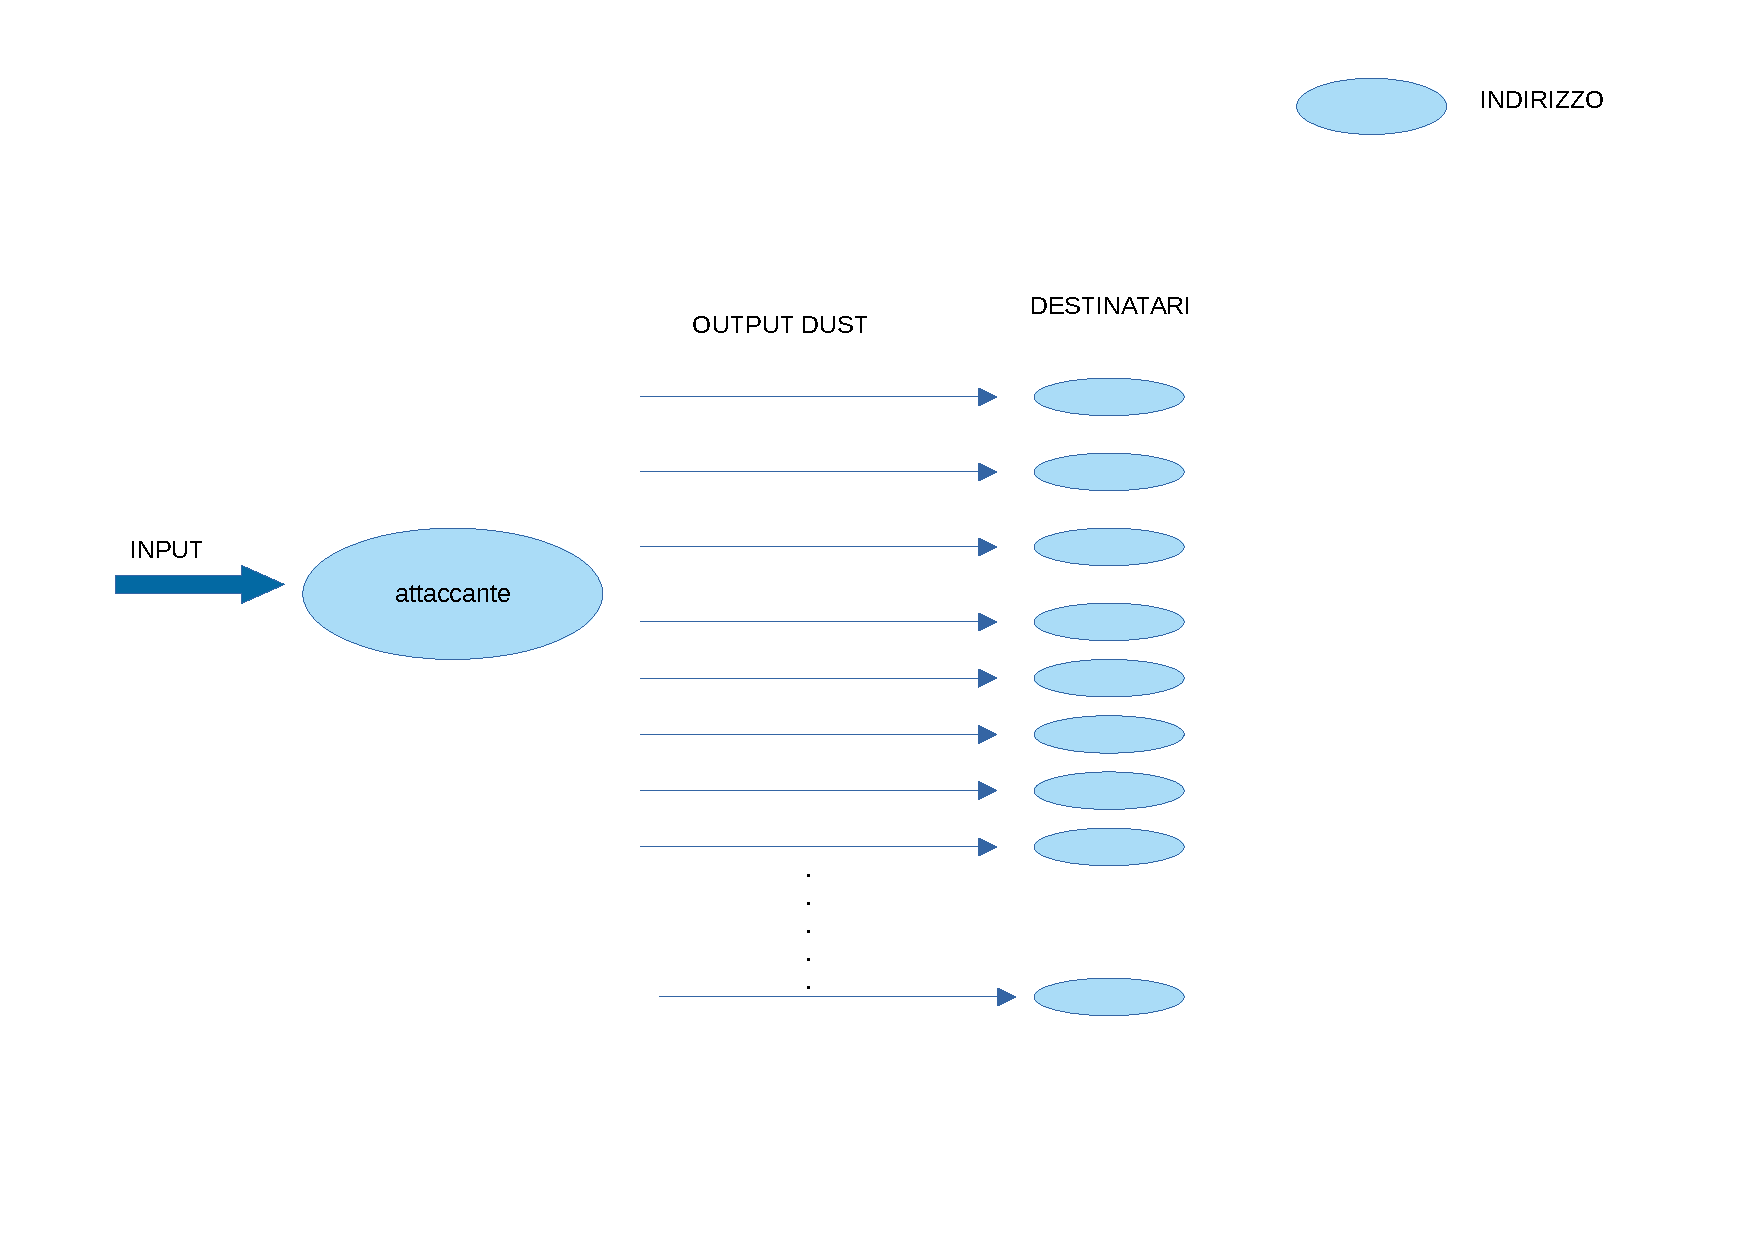
\includegraphics[scale=0.5, trim = 1cm 5cm 0cm 0cm, clip]{Images/dust_attack.pdf}
    \caption{Schema Dust Attack}
    \label{fig:Dust_attack}
\end{figure}
\FloatBarrier
Possono esserci due possibili esiti del Dust Attack: 
    \begin{enumerate}
        \item attacco di successo;
        \item attacco fallito.
    \end{enumerate}
    
Nel primo caso, mostrato in figura \ref{fig:success}, la vittima genera una transazione in cui spende l'importo dust ricevuto insieme ad almeno un altro dei suoi address. 

Questi address quindi sono collegati tra loro dalla euristica sui multi-input, ed é possibile capire che appartengano ad uno stesso utente. Se l'attaccante successivamente scopre le informazioni personali, come nome o email, del proprietario di uno di questi address automaticamente scopre che tutti gli altri address hanno lo stesso proprietario. Inoltre é possibile tracciare l'attività di un utente e non solo di un singolo address.
\begin{figure}[h!]
    \centering
    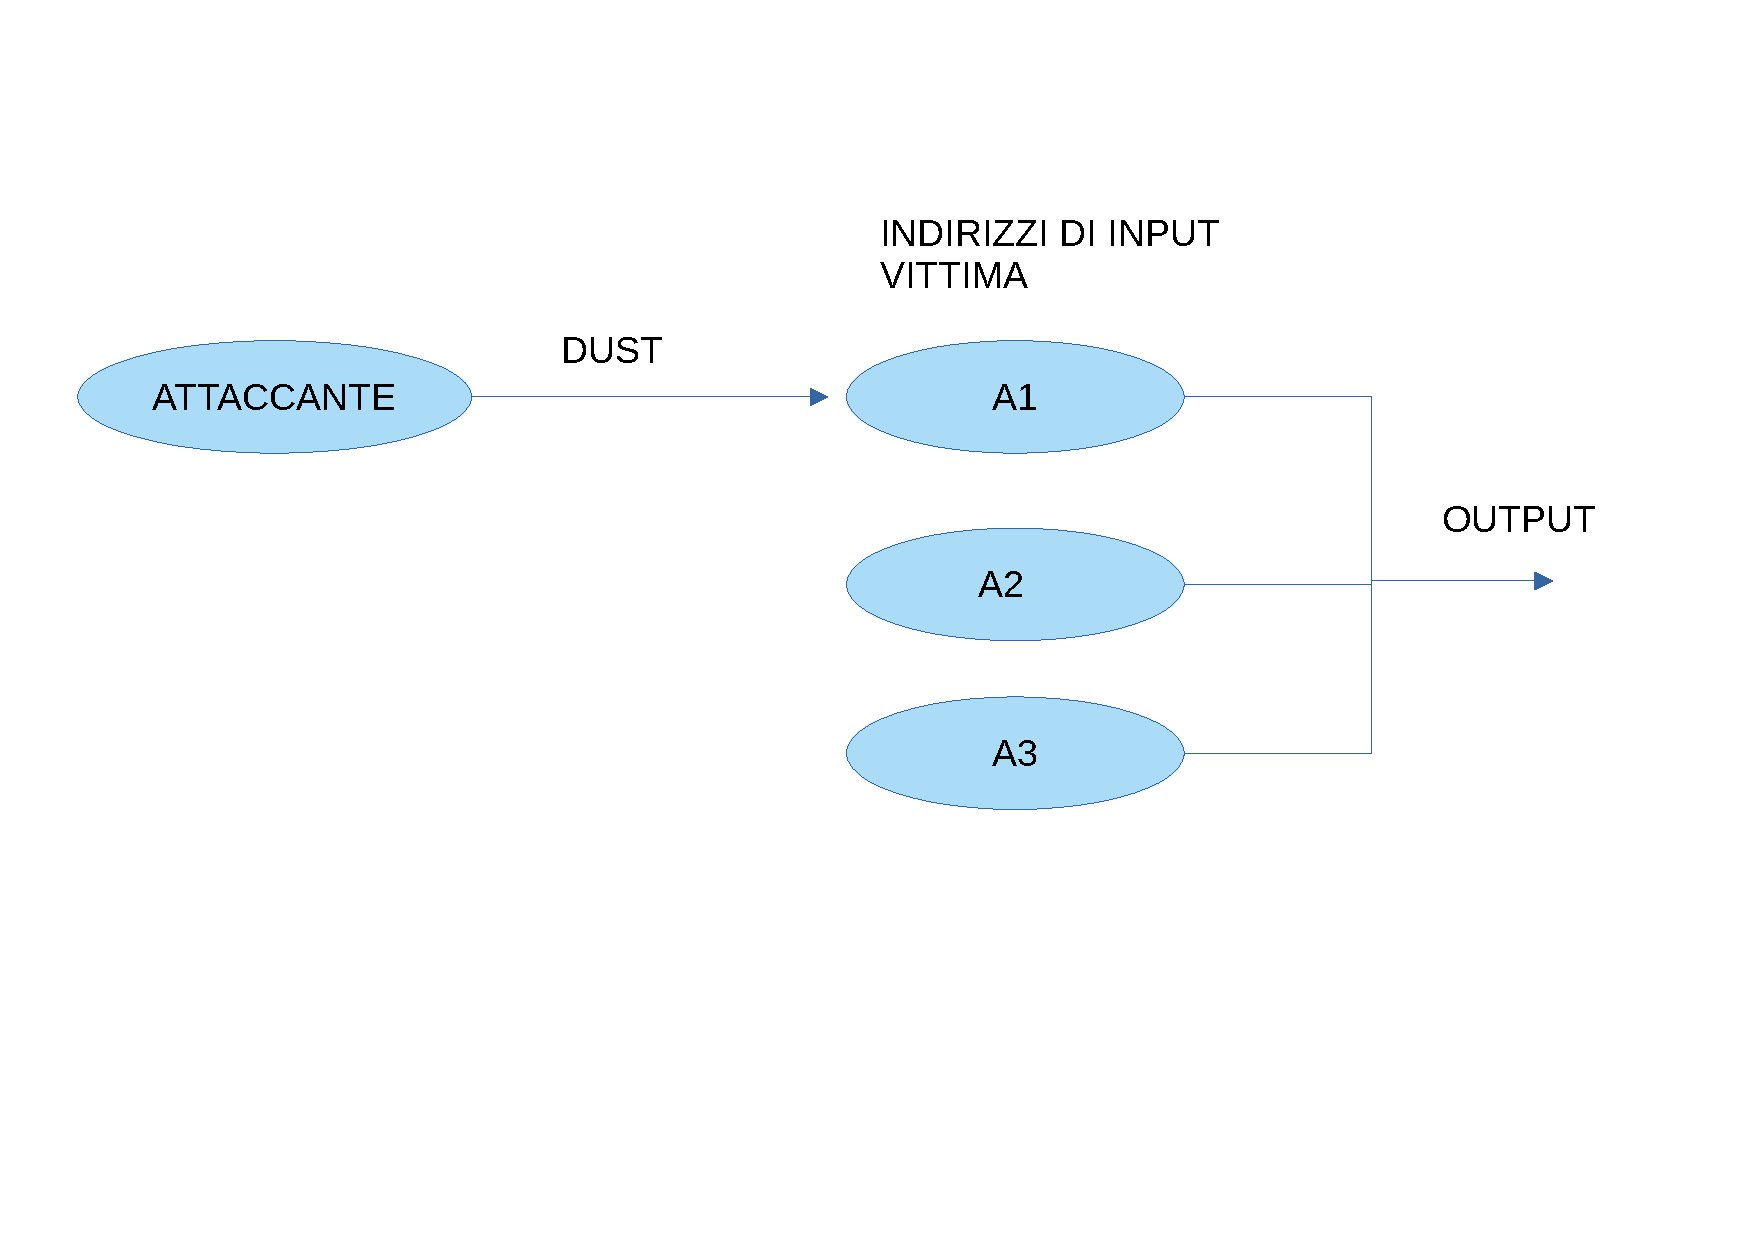
\includegraphics[scale=0.5,trim = 1cm 6cm 0cm 3cm, clip]{Images/successo.pdf}
    \caption{Schema di Dust Attack di Successo: l'address del dust viene speso con altri address}
    \label{fig:success}
\end{figure}
\FloatBarrier
Esistono invece due possibili motivi per cui un Dust Attack può fallire. In figura \ref{fig:fallito} vengono schematizzati questi due possibili esiti.

Nel primo schema la vittima spende il dust ricevuto, ma utilizza una transazione i cui input si riferiscono ad UXTO relativi all'address in cui é stato depositato il dust. In questo caso l'attaccante non ricava alcuna informazione perché non riesce nell'intento di provocare l'unione di address diversi di un utente nella medesima transazione. Nel secondo schema invece la vittima non spende il dust, troncando sul nascere l'attacco. 

Il Dust Attack, in generale, risulta più efficace soprattutto se il dust é diretto verso gli address che hanno un bilancio complessivo pari a zero proprio perché obbliga la vittima a spendere la cifra ottenuta con altri suoi address diversi.

\begin{figure}[h!]
    \centering
    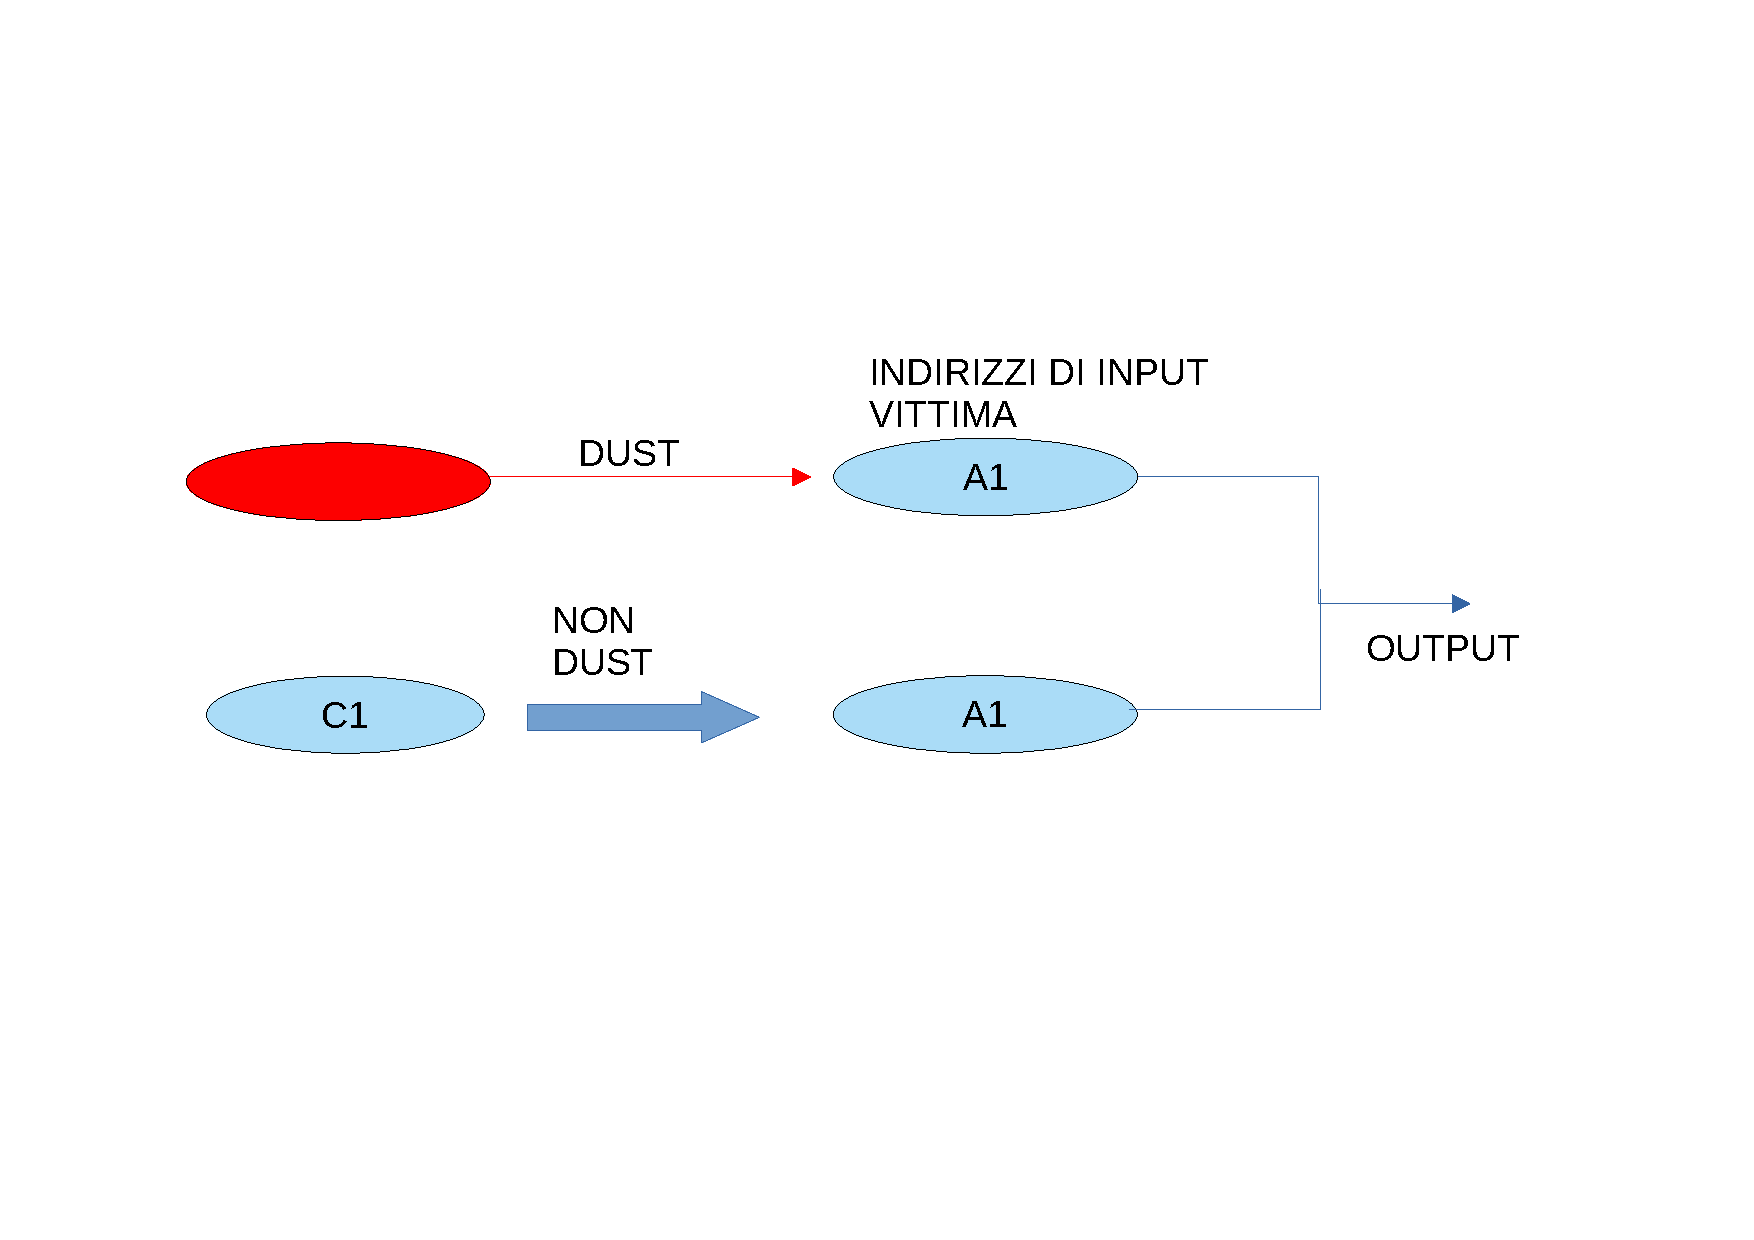
\includegraphics[scale=0.5, trim = 1cm 6cm 0cm 3cm, clip]{Images/fallito2.pdf}
    (a)
    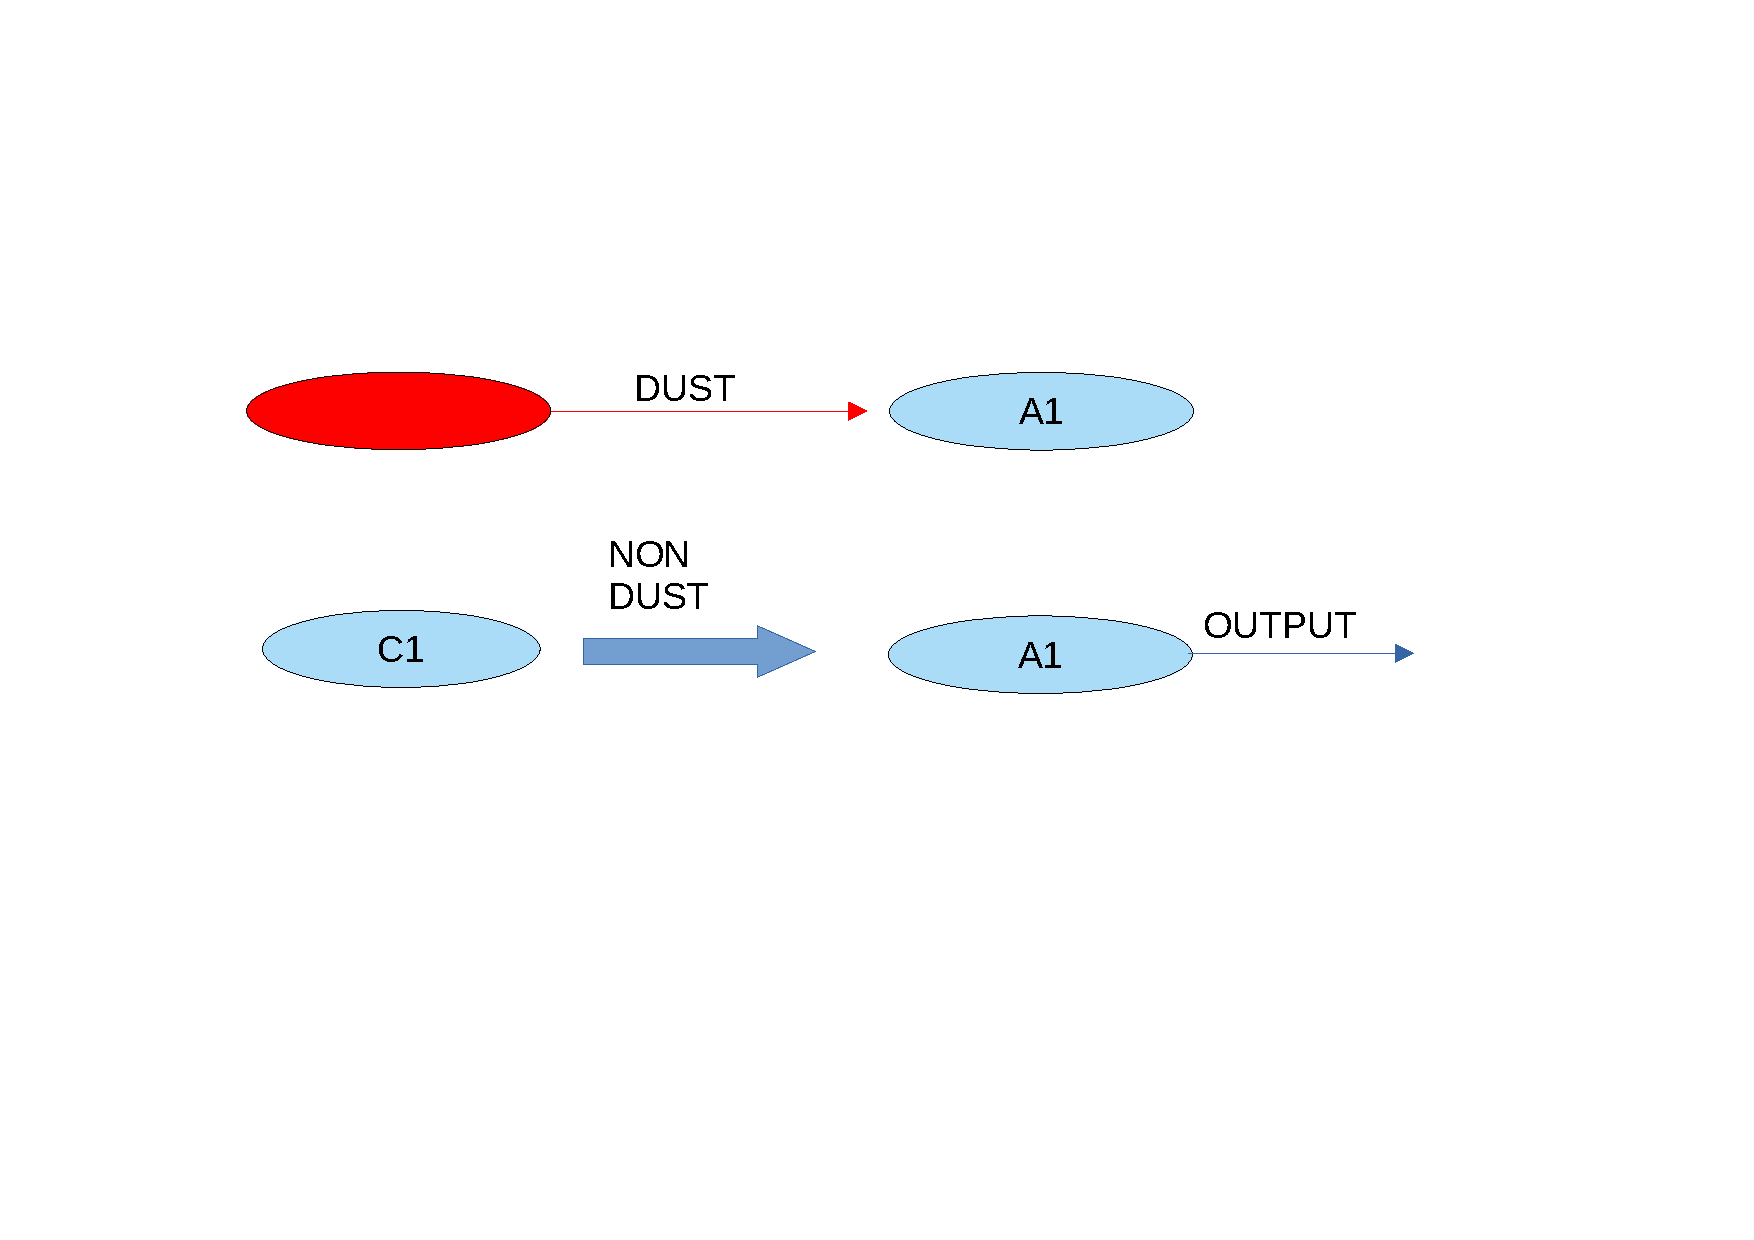
\includegraphics[scale=0.5, trim = 1cm 7cm 0cm 2cm, clip]{Images/fallito1.pdf}
    (b)
    \caption{Schema di Dust Attack Fallito. La vittima spende il dust con un solo address(a), la vittima non spende il dust(b)}
    \label{fig:fallito}
\end{figure}
\FloatBarrier

é importante notare che lo scopo del Dust Attack non é quello di rubare fondi di altri utenti né quello di scoprire informazioni personali, per esempio nome e cognome, della vittima. Permette, invece, di rompere lo pseudo-anonimato degli address, ovvero l'appartenenza di address differenti ad uno stesso utente. Questa informazione può essere usata in seguito per effettuare attacchi elaborati e più pericolosi.

In generale il Dust Attack non necessariamente é legato a phishing o estorsioni ma potrebbe essere usato dalle autorità per tenere traccia degli utenti ed eventualmente rilevare attività illegali.

Infatti una volta ottenuto un cluster di address é possibile tracciare l'attività di un singolo utente e non più di un singolo address. Le autorità potrebbero notare che certi utenti interagiscono con address legati a mercati neri, e quindi indagare ulteriormente per scoprire l'identità di queste persone.

Uno dei punti fondamentali é legare informazioni personali, come e-mail, nome ed altro, ad un address Bitcoin. In molti casi sono gli utenti stessi che pubblicano sui forum i loro address, in altre situazioni invece é possibile sfruttare gli \emph{exchange} come Coinbase.

Gli exchange sono servizi che permettono lo scambio tra criptovalute e valute tradizionali basandosi sul valore di mercato della criptovaluta. In exchange reputati affidabili, come Coinbase, é necessario creare un account fornendo informazioni personali come nome, cognome, email ed altro e, una volta registrati, viene creato un wallet associato a quel particolare account. Anche se, poiché gli exchange sono vittime appetibili di attacchi hacker, molti utenti trasferiscono i loro bitcoin su address appartenenti a software wallet. Una volta che un utente effettua un deposito dal wallet, vittima di Dust Attack, ad un account exchange l'attaccante può collegare gli address al proprietario. Ed una volta ottenuta l'identità del proprietario, l'attaccante può eseguire elaborati attacchi di phishing oppure può estorcere denaro minacciandolo di rivelare a tutti l'informazione ottenuta. 

Per fortuna, il Dust Attack non é particolarmente difficile da contrastare, nel paragrafo successivo verranno mostrati due metodi per difendersi da questo tipo di attacco.

\subsection{Contromisure al Dust Attack}

Due metodi che un utente che ha ricevuto un importo dust può utilizzare per contrastare il Dust Attack sono:
    \begin{enumerate}
        \item non spendere l'importo dust ricevuto; 
        \item utlizzare servizi di ``dust collecting". 
    \end{enumerate}
    
La prima soluzione, semplice ed efficace, permette di troncare l'attacco sul nascere. Infatti se il dust non viene speso l'attaccante non potrà mai collegare address diversi dello stesso utente.  Diversi software wallet implementano questo metodo; per esempio Samurai Wallet \footnote{fonte:\url{https://twitter.com/samouraiwallet/status/1055345822076936192?lang=en}}, nel 2018, consigliò ai suoi utenti, possibili vittime di Dust Attack,  di contrassegnare come ``do not spend" ogni output dust ricevuto.

La seconda soluzione riguarda i servizi di ``dust collecting", come, ad esempio, Dust-B-Gone \cite{Dbg}.
Dust-B-Gone, ideato da Peter Todd già nel 2012, era un servizio che permetteva di disfarsi del dust, non lasciando il dust ricevuto come UTXO, ma trasformandolo in fee per i miner. Il programma generava un'unica transazione alla quale potevano cooperare più utenti. Ogni utente inseriva tra gli input della transazione l'importo dust ricevuto così da potersene liberare. Allo stesso tempo questo servizio proteggeva gli utenti da una possibile de-anonimizzazione, poiché address diversi di una transazione potevano appartenere ad utenti diversi. Un attaccante quindi non avrebbe mai potuto collegare questi address, o comunque ne avrebbe ricavato una falsa informazione.
Nonostante la solida idea di base, notiamo che questo servizio é stato chiuso nel 2016 per vari motivi, tra cui il suo scarso utilizzo \footnote{fonte: \url{https://twitter.com/SamouraiWallet/status/1293659938422652935}} . 